\usetikzlibrary{decorations.markings,arrows.meta,bending, patterns}

\subsection*{Page 124, Problem 1 (Worked with David LaRoche)}
\vspace{15pt}
\begin{proof}
    \vspace{-10pt}\;
    \begin{enumerate}[label = (\alph*)]
        \item To triangulate the cylinder, identify the edges of complex $K$ embedded in $\E^3$:
        \begin{center}
            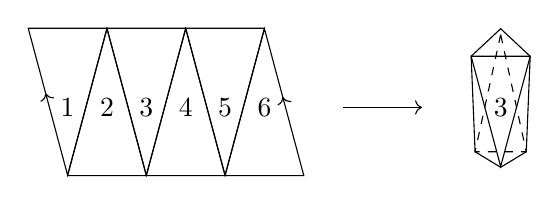
\begin{tikzpicture}
                \tikzset{->-/.style={decoration={
                markings,
                mark=at position #1 with {\arrow{<}}},postaction={decorate}}}

                \draw[xshift = -.5cm, yshift = .14cm, ->-=.4] (60:1) -- (120:1) -- (270:1) -- cycle (0, -.14) node {1};

                \draw[xshift = 0cm] (240:1) -- (90:1) -- (300:1) -- cycle (0, 0) node {2};

                \draw[xshift = .5cm, yshift = .14cm] (60:1) -- (120:1) -- (270:1) -- cycle (0, -.14) node {3};

                \draw[xshift = 1cm] (240:1) -- (90:1) -- (300:1) -- cycle (0, 0) node {4};

                \draw[xshift = 1.5cm, yshift = .14cm] (60:1) -- (120:1) -- (270:1) -- cycle (0, -.14) node {5};

                \draw[xshift = 2.0cm,  ->-=.6] (240:1) -- (90:1) -- (300:1) -- cycle (0, 0) node {6};

                \draw[black, ->] (3,0) -- ++ (1cm, 0);

                \draw[xshift = 5.0cm] (60:.75) -- (120:.75) -- (270:.75) -- cycle (0,0) node {3};

                \draw[xshift = 5.0cm] (60:.75) -- (90:1) -- (120:.75) -- (240:.65) -- (270:.76) -- (300:.65) -- (60:.75);

                \draw[xshift = 5.0cm, dashed] (90:.925) -- (240:.65) -- (300:.65) -- cycle;
            \end{tikzpicture}
        \end{center}
        This will leave a through-hole in the cylinder which is homeomorphic to the cylinder $S^1 \times [0,1].$

        \item To triangulate the klein bottle, we can simply stitch together 3 such cylinders from above in a `4'-like shape using the following identification:
        \begin{center}
            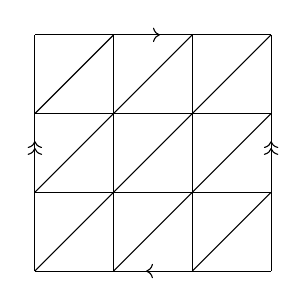
\begin{tikzpicture}
                \tikzset{->-/.style={decoration={
                markings,
                mark=at position #1 with {\arrow{<}}},postaction={decorate}}, ->>-/.style={decoration={
                markings,
                mark=at position #1 with {\arrow{>>}}},postaction={decorate}}}
                
                \draw (2,0) -- (3,1);
                \draw (1,0) -- (3,2);
                \draw (0,0) -- (3,3);
                \draw (0,1) -- (2,3);
                \draw (0,2) -- (1,3);
                \draw (1,0) -- (1,3);
                \draw (2,0) -- (2,3);
                \draw (0,1) -- (3,1);
                \draw (0,2) -- (3,2);
                \draw[->-=.5] (0,0) -- (1,0) -- (2,0) -- (3,0);
                \draw[->-=.5] (3,3) -- (2,3) -- (1,3) -- (0,3);
                \draw[->>-=.55] (0,0) -- (0,1) -- (0,2) -- (0,3);
                \draw[->>-=.55] (3,0) -- (3,1) -- (3,2) -- (3,3);
            \end{tikzpicture}
        \end{center}
        This was derived normally but confirmed precisely by Figure 6.14 in the book.

    \item Now, to triangulate the double torus, we will use the piece-by-piece construction of two punctured pre-identification toruses stitched together via a cylinder, i.e. not exactly but nearly 2 connect sums:
        \begin{center}
            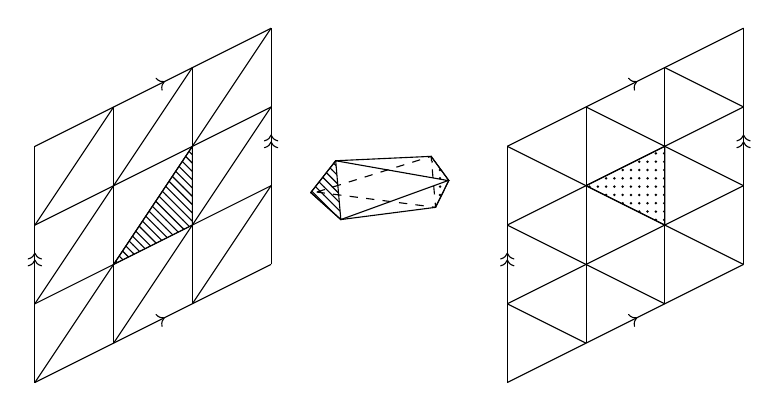
\begin{tikzpicture}
                \tikzset{->-/.style={decoration={
                markings,
                mark=at position #1 with {\arrow{>}}},postaction={decorate}},
                 ->>-/.style={decoration={
                markings,
                mark=at position #1 with {\arrow{>>}}},postaction={decorate}}}


                \draw (0,1) -- (3,2.5);
                \draw (0,2) -- (3,3.5);
                \draw (1,.5) -- (1,3.5);
                \draw (2,1) -- (2,4);
                \draw[->-=.55] (0,0) -- (3,1.5);
                \draw[->-=.55] (0,3) -- (3,4.5);
                \draw[->>-=.55] (0,0) -- (0,3);
                \draw[->>-=.55] (3,1.5) -- (3,4.5);

                \draw (0,2) -- (1,3.5);
                \draw (0,1) -- (2,4);
                \draw (0,0) -- (3,4.5);
                \draw (1,.5) -- (3,3.5);
                \draw (2,1) -- (3,2.5);

                \draw[pattern = north west lines] (1, 1.5) -- (2,2) -- (2,3) -- cycle;

                \begin{scope}[xshift = 4.5cm, yshift = 2.5cm, rotate = 95]

                    \draw(60:.75) -- (120:.75) -- (270:.75) -- cycle (0,0);

                    \draw(60:.75) -- (90:1) -- (120:.75) -- (240:.65) -- (270:.76) -- (300:.65) -- (60:.75);
    
                    \draw[dashed] (90:.925) -- (240:.65) -- (300:.65) -- cycle;

                    \draw[pattern = north west lines] (60:.75) -- (90:1) -- (120:.75);

                    \draw[pattern = dots] (240:.65) -- (270:.76) -- (300:.65);
                \end{scope}

                \begin{scope}[xshift = 6cm]
                    \draw (0,1) -- (3,2.5);
                    \draw (0,2) -- (3,3.5);
                    \draw (1,.5) -- (1,3.5);
                    \draw (2,1) -- (2,4);
                    \draw[->-=.55] (0,0) -- (3,1.5);
                    \draw[->-=.55] (0,3) -- (3,4.5);
                    \draw[->>-=.55] (0,0) -- (0,3);
                    \draw[->>-=.55] (3,1.5) -- (3,4.5);
    
                    \draw (2,4) -- (3,3.5);
                    \draw (1,3.5) -- (3,2.5);
                    \draw (0,3) -- (3,1.5);
                    \draw (0,2) -- (2,1);
                    \draw (0,1) -- (1,.5);
    
                    \draw[pattern = dots] (1, 2.5) -- (2,3) -- (2,2) -- cycle;
                \end{scope}
            \end{tikzpicture}
        \end{center}
        Note that the identification arrows on the left torus are separate from the arrows on the right torus. Also, identification arrows from the cylinder's lined triangle onto the torus's missing triangle are left out. As are the ones for the resected and dotted left torus piece. Moreover, note that the left and right toruses will fold out AWAY from the cylinder. This triangulation preserves the hollow inside but a homeomorphism can be easily constructed to shrink this cylinder away leaving just the double torus (not that this is needed, but for visual clarity that it is indeed the double torus).
    \end{enumerate}
\end{proof}

\subsection*{Page 131, Problem 18 (Worked with David LaRoche)}
\vspace{15pt}
\begin{proof}
    \vspace{-10pt}
    Take the set $S = \{\langle f\rangle \mid f\colon |K| \to |L|\}$ for simplicial complexes $K, L$. $K, L$ are finite (per the definition) so suppose, without loss of generality, they have $m,n$ vertices respectively. Further recall that the image of $K$'s vertices under a simplicial map linearly determine the rest of the map. Since each vertex of $K$ must map to some vertex of $L$, there are at most $n^m$ possible maps.

    By the simplicial approximation theorem, any map $f\colon |K| \to |L|$ can be approximated by some simplicial approximation $s \colon |K^j| \to |L|$ for some $j \in \Z^+\cup\{0\}.$ Note $K^j$ has a finite number of vertices so the number of possible simplicial maps, as disccused above, is always finite, namely $n^{(\#\text{ of vertices of $K^j$})}$. This means there are a finite number of possible homotopy classes per $j$-th subdivision of $K$ (even with extensive double-counting). 
    
    Because any function has a simplicial approximation for large enough $j$, all homotopy classes will eventually be covered for $j = 0,1,2\ldots.$. Therefore, we can just count the finite number of all possible homotopy maps per subdivision. This consequently bounds $|S|$ above by a countable sum of finite values making the set of all homotopoy classes of functions from $|K| \to |L|$ countable.
\end{proof}